\documentclass[letterpaper,10pt,twocolumn]{article}

\usepackage{algorithm}
\usepackage{algpseudocode}
\usepackage{amsmath}
\usepackage{amssymb}
\usepackage{amsthm}
\usepackage{fullpage}
\usepackage{romannum}
\usepackage{xcolor}
\usepackage{graphicx}
\usepackage{wasysym}
\usepackage{pifont}
\usepackage[hidelinks]{hyperref}

\setlength{\textwidth}{6.5in}
\setlength{\textheight}{9in}
\setlength{\columnsep}{.25in}
\date{}

\def\protocol/{FAW}

\begin{document}

\title{Proof of the \protocol/ Protocols}

\pagenumbering{arabic}
\maketitle

In this document, we demonstrate the correctness of the \protocol/ protocol (\S\ref{sec:faw}), its variant for two-phase commit (2PC) (\S\ref{sec:2pc}) and the \textsc{RainTx} transaction protocol (\S\ref{sec:raintx}).
Also note two \emph{errata} of the original paper (\S\ref{sec:errata}).

\section{\protocol/ Write Procedure}
\label{sec:faw}

The form of the three-phase update procedure results from safety constrains.
We first establish a \emph{generic} write procedure that models \emph{all possible} write paths.
Then we enforce the safety constrains on the generic model and show that the \protocol/ write procedure is necessary and optimal. 

\subsection{Generic Write Model}

We consider a stripe of $n$ chunks using a $k$-of-$n$ fault tolerance scheme.
A write request modifies $u$ chunks (including the $m$ redundant chunks).
A traditional logging method has to duplicate all $u$ chunks, while our procedure allows $\delta$ chunks to be updated in-place, saving $\delta$ chunk writes.

After logging and updating $u - \delta$ chunks, the remaining steps of the write procedure can be viewed as a repeat of a step that in-place updates some of the $\delta$ chunks.
We assume, in the $i$th step, $\epsilon_i$ chunks are updated in-place in parallel, and before that step, $d_i$ chunks have been updated in-place by previous steps ($d_1=0$ denotes the first step).
Therefore, $d_{i+1} = d_i + \epsilon_i$, for $i \in \mathbb{N}^{+}$. If $d_i + \epsilon_i < \delta$, that means not all $\delta$ chunks can be updated in the $i$th step, so we have to do a next step; otherwise, the write procedure ends.
Various write paths result from choosing a different $\epsilon$ in every step.
A write path consists of a series of steps $(0, e_1), (d_2, \epsilon_2), ..., (\delta, 0)$: in the first step, we update $e_1$ chunks while no chunks have been updated; in the second step, we update $\epsilon_2$ chunks while $d_2$ chunks (which equals to $\epsilon_1$ in this step) have been updated; so on and so forth; finally, we have updated all $\delta$ chunks and thus we should update no chunks in the end step.
We visualize the steps in an $\epsilon$-dimensional space (see Figure~\ref{fig:d-e-space}).
A point in the figure represents a step in a write path.

\subsection{Optimization and Constrains}

We formalize the problem of finding the optimal and safe write procedure of \protocol/ as an optimization problem. 
In this optimization problem, the \emph{objective} is to maximize $\delta$, while the \emph{constraints} are to guarantee the safety of data.

\noindent
\textbf{Constraints.} To express the constraints, we have to count the chunks of different versions, as summarized in Table~\ref{tab:states}.
Note that a chunk is regarded as holding both new and old versions (``new/old'') when it is logged and updated; also, if it does not change at all in the write
path (``not updated''), it is regarded as holding both versions. A chunk
holds none (``--'') if it is being updated in-place.

As described in the original paper, we assume a distribution of $f$ is a tuple $(f_0, f_1, f_2)$, where $f_0$ failures destroy
chunks holding both versions, $f_1$ failures destroy old-version only chunks,
and $f_2$ destroy new-version only chunks. Then, the invariant is equivalent to
satisfying one of the following two constraints.

\begin{table}[!b]
\centering
\begin{tabular}{l|c|c}
\hline
State & \# of chunks & Version \\
\hline
not to be updated & $n - u$ & new/old \\
logged and updated & $u - \delta$ & new/old \\
updated in-place & $d_i$ & new \\
being-updated in-place & $\epsilon_i$ & -- \\
not-yet-updated in-place & $\delta - d_i - \epsilon_i$ & old \\
\hline
\end{tabular}
\caption{Chunk states. A chunk holds the old or/and the new version of data.  }
\label{tab:states}
\end{table}

\emph{C1 -- the number of old-version chunks is greater than or equal to $k$}: The number of old-version chunks is $(n -
u) + (u - \delta) + (\delta - d_i - \epsilon_i)$, as Table~\ref{tab:states}
lists. Among all $f$ failures, $f_0 + f_1$ destroy old-version chunks.
So, we must have $(n - u) + (u - \delta) + (\delta -
d_i - \epsilon_i) - (f_0 + f_1) \ge k$ to recover using \emph{roll-back}.

\emph{C2 -- the number of new-version chunks is greater than or equal to $k$}: Similarly, summing up all new-version
chunks as in Table~\ref{tab:states} and considering $f_0 + f_2$ failures that
destroy new-version chunks, we must have $(n - u) + (u - \delta) + d_i
- (f_0 + f_2) \ge k$ to recover using \emph{roll-forward}.

We construct the worst-case failure distribution by assuming an
\emph{adversary} who attempts to make best use of the $f$
failures to maximize damaged data.  Our protocol and the adversary are
\emph{gaming} against each other.

The first priority of the adversary must be to increase $f_0$ because one such
failure can cause damage to \emph{both} versions anyway.  Consequently, if the
number of chunks with both versions is larger than $f$, the adversary must set
$f_0 = f$, and $f_1 = f_2 = 0$. As a result, C1 becomes:
\begin{equation}
\epsilon_i \le -d_i + (m - f).
\label{eq:roll-back-constraint}
\end{equation}

And C2 becomes:
\begin{equation}
d_i \ge \delta - (m - f).
\label{eq:roll-forward-constraint}
\end{equation}

Otherwise (the number of chunks with both versions is less than
$f$), the adversary would maximize $f_0$ by setting it to the number
of chunks with both versions, i.e., $f_0 = (n - u) + (u - \delta)$.
Since $f_0$ is determined, C1 becomes $f_1 \le
m - (n - \delta) - d_i - \epsilon_i$. In addition, substituting $f - f_0 - f_1$
for $f_2$, C2 becomes $f_1 \ge \delta - (m - f) - d_i$.
The adversary must seek $f_1$ within the scope $(m - (n - \delta) - d_i -
\epsilon_i, \delta - (m - f) - d_i)$ so that neither C1 nor C2 is satisfiable.
Therefore, we have to ensure the scope is empty.  As the value of $f_1$ is
discrete, that requires $m - (n - \delta) - d_i - \epsilon_i \ge \delta - (m -
f) - d_i - 1$, which is:
\begin{equation}
\epsilon_i \le (2m - f) - n + 1.
\label{eq:discretionary}
\end{equation}

\begin{figure}[!t]
  \centering
  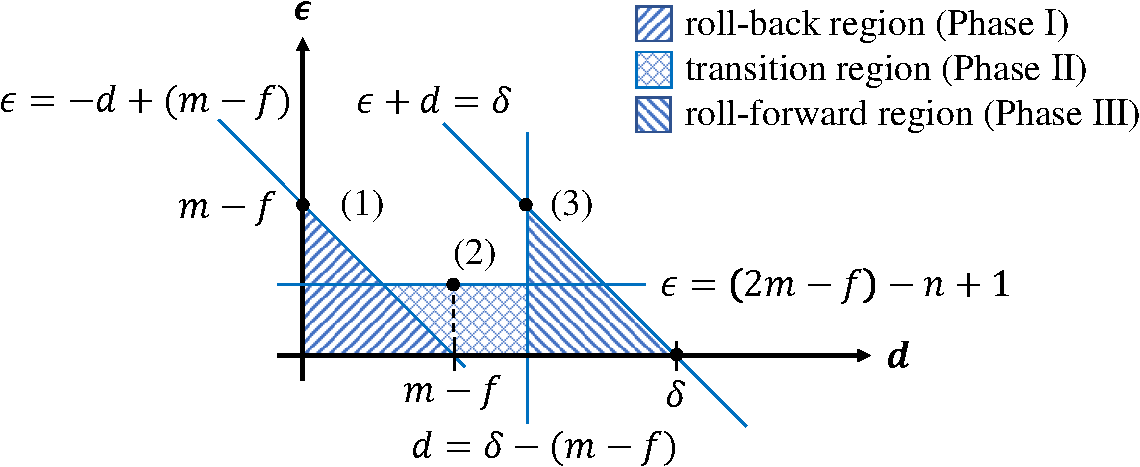
\includegraphics[width=\linewidth]{figures/d-e-space}
  \caption{\protocol/ steps in a $d-\epsilon$ space. A point $(d, \epsilon)$
means one step to update $\epsilon$ chunks when $d$ chunks have been updated.
Constraints produce feasible regions (e.g., the left side of the line $\epsilon
= -d + (m - f)$ satisfies $\epsilon \le -d + (m - f)$, which is
Inequality~\ref{eq:roll-back-constraint}). Points (1) -- (3) represent three
steps of a write path. \vspace{-1em}}
  \label{fig:d-e-space}
\end{figure}

In Figure~\ref{fig:d-e-space}, we color all feasible $(d_i, \epsilon_i)$ points
that satisfy the constraints. The left triangle region always supports
roll-back in \emph{any distribution} of failures, because any point/step
therein can survive the most adversarial case which leads to
Inequality~\ref{eq:roll-back-constraint}. Similarly, any point/step in the right triangle region is
constantly recoverable by roll-forward. Between them may exist a
\emph{transition region} where we cannot say for sure whether recovery will be via rolling forward or backward. 
One or the other will surely work, and the exact choice depends on the failure distribution (particularly, the choice of $f_1$ as
discussed for Inequality~\ref{eq:discretionary}).

\subsection{Procedure and Proof}

Having the model and constraints, we now solve the optimization problem: find the
maximum $\delta$ so that there is a safe write procedure.  A write procedure is
safe as long as every step is recoverable, i.e., located in the
feasible regions in Figure~\ref{fig:d-e-space}.  As long as $\epsilon = (2m -
f) - n + 1 \ge 1$, i.e., $n \le 2m - f$, all three regions connect. That means
any step can find a feasible $\epsilon$ until $d = \delta$ which is the end of
a write path. If so, there is no safety restriction on the value of $\delta$,
which can be up to $u$.

Otherwise, when $n > 2m - f$, the transition region is empty. But if the
roll-back region and the roll-forward region connect, a write path 
always exists. Thus, we need
$\delta - (m - f) \le m - f$, i.e., $\delta \le 2(m
- f)$. All in all, the maximal $\delta$ is as follows.
\begin{equation}
\delta_{\max} =
\begin{cases}
u, & \text{if } n \le 2m-f;\\
\min\{2(m-f), u\}, & \text{otherwise.}
\end{cases}
\label{eq:delta}
\end{equation}

Next, we determine the optimal write procedure.
As Figure~\ref{fig:d-e-space} shows, when $d = 0$, we take the first step. To reduce the overall latency, we update as many chunks as possible in parallel.
As a result, this step will reach from $d=0$ to $d=m-f$, bypassing the entire roll-back region.
This step corresponds to Phase~\Romannum{1} of \protocol/.
Hence, the number of chunks to update in this phase is $s_1=m-f$.
Then, we go through the transition region where $\epsilon = (2m - f) - n + 1$.
Different from a triangle-shaped region, it is possible we need more than one
step to get across the region.
These steps make Phase~\Romannum{2}.
Finally, we can go through the roll-forward region in a single step with $s_3=m-f$ in Phase~\Romannum{3}.
In conclusion, \protocol/ produces a safe write procedure whose every step is recoverable, with maximum $\delta$ as well as minimal latency (steps).

\section{\protocol/-2PC Protocol}
\label{sec:2pc}

We aim to prove that, after a logged Phase~\Romannum{2}, the stripe is recoverable by both roll-back and roll-forward.

If Phase~\Romannum{2} does not exist, i.e., $\delta \le 2(m-f)$, the roll-back region and the roll-forward region in Figure~\ref{fig:d-e-space} overlap.
The state of the chunks after Phase~\Romannum{1} is $(m-f,0)$.
Note that a point with $\epsilon=0$ denotes a state (or a ``step'' without updating any chunk).
The point falls in both the roll-back region and the roll-forward region, so the state is recoverable by both roll-back and roll-forward.

Next, we consider the case $\delta > 2(m-f)$.
Phase~\Romannum{2} updates $s_2=\delta-2(m-f)$ chunks in-place.
\protocol/-2PC requires the $s_2$ chunks to be logged as well, so only the rest $2(m-f)$ chunks avoid logging.
Accordingly, the state after Phase~\Romannum{2} is as Table~\ref{tab:states-2} lists.
We examine the state with C1 and C2.
Both C1 and C2 translate to $n-(m-f) \ge k$.
In the worst case, all $f$ failures destroy the old-version/new-version chunks for C1/C2, so C1/C2 becomes $n-(m-f)-f \ge k$, i.e., $n-m \ge k$.
Since $n-m=k$ by definition, the inequality is constantly true.

Overall, after a logged Phase~\Romannum{2} (no matter whether it is empty), the
chunks can always roll back or roll forward, if 2PC requires either.

\begin{table}[!ht]
\centering
\begin{tabular}{l|c|c}
\hline
State & \# of chunks & Version \\
\hline
not to be updated & $n-u$ & new/old \\
logged and updated & $u - 2(m-f)$ & new/old \\
updated in-place & $m-f$ & new \\
being-updated in-place & $0$ & -- \\
not-yet-updated in-place & $m-f$ & old \\
\hline
\end{tabular}
\caption{Chunk states after a logged Phase~\Romannum{2}.}
\label{tab:states-2}
\end{table}



\section{\textsc{RainTx} Protocol}
\label{sec:raintx}

\section{Errata}
\label{sec:errata}

\begin{itemize}

\item Figure~5(b) of the original paper should be replaced with Figure~\ref{fig:raintx-commit}.
The original figure does not match our description of Step~\ding{196} in the text, though it is also a correct protocol -- it shows an optimization we planned but did not get enough time to implement before the paper submission.
The optimization is to unlock primaries as early as possible without waiting for the coordinator's notifications.
Note that our evaluation of \textsc{RainTx} follows Figure~\ref{fig:raintx-commit} without the optimization.
Its Step~\ding{196} is similar to Step~\ding{196} of FaRM.

\begin{figure}[!h]
  \centering
  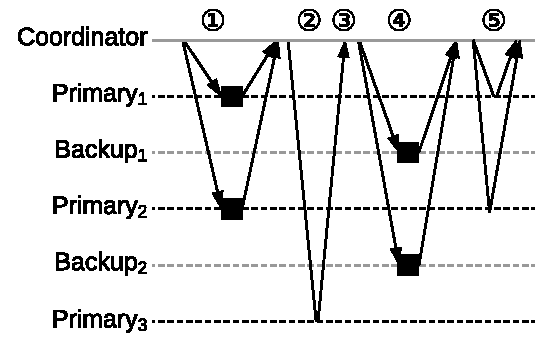
\includegraphics[width=0.7\linewidth]{figures/raintx-commit}
  \caption{The commit protocol of \textsc{RainTx}.}
  \label{fig:raintx-commit}
\end{figure}

\item In Figure~8(a) of the original paper, ``FM-thr'' and ``RX-thr'' should be swapped.
The throughput of \textsc{RainTx} (RX-thr) is higher than that of FaRM (FM-thr).

\end{itemize}

\end{document}
